\subsection{Комбинаторные неразрешимые задачи}

$U_{TM} = \{ \left< m, x \right> \mid n$ для $x \}$

Докажем, что $U_{TM}$~--- не разрешим.

\begin{theorem}
    $\{\left< \Gamma x \right> \mid S \implies^* x\}$~--- не разрешаим.
\end{theorem}

\subsubsection*{Gamma--грамматика класса 0}

$\alpha \to \beta$, $\alpha \in N^+ $, $\beta \in \left( N \cup \Sigma\right)$.

Например, $0^n 1^n 2^n$~--- не К.С.

Разрешим его в грамматике класса 0.

\begin{itemize}
    \item $S \to XYZ$
    \item $Y \to \varepsilon$
    \item $Y \to ABCY$
    \item $BA \to AB$
    \item $CA \to AC$
    \item $CB \to BC$
    \item $XA \to 0X$
    \item $X \to P$
    \item $PB \to 1P$
    \item $P \to Q$
    \item $QC \to 2Q$
    \item $QZ \to \varepsilon$.
\end{itemize}

\begin{theorem}
    $L$~--- перечислим $\iff$ $L$~--- пораждается граматикой класса 0.
\end{theorem}
\begin{proof}
    Пусть есть маширна тьюринга, которая допускает слово $m$.\\
    $q_0 = \#_s x \vdash q_1 \vdash q_2 \vdash \dots \vdash q_t = \alpha \#_y \beta$.

    \[ S \underbrace{\implies^{*}}_{\begin{array}{l}S \to \land Y \$, \\Y \to Z \#_Y Z,\\ Z \to cZ,\\ Z \to \varepsilon\end{array}}  \land \alpha \#_y \beta \$ \underbrace{\implies \land q_{t-1} \$ \implies \dots \implies}_{\begin{array}{l}\delta(p, c) = (q, d, \leftarrow),\\ \#_q  ad \to a \#_p c\end{array}} \land q_1 \$ \underbrace{ \implies}_{\land \#_s \to \sim} \land q_0 \$ \implies^{*} x \sim \$ \implies x . \]
\end{proof}

\begin{problem}
    [Проблема соответствия поста (PCP)]

    $\mathrm{PCP} =$\\
    $ = \{ \left< (\alpha_1, \beta_1), (\alpha_2, \beta_2), \dots, (\alpha_n, \beta_n) \right> \mid \exists i_1, i_2, \dots, i_k ~:~  \alpha_{i_1} \dots\alpha_{i_k} = \beta_{i_1}\dots\beta_{i_k} \}$.

    $U_{TM} \leqslant \mathrm{PCP}_1 \leqslant \mathrm{PCP}$.

    $\mathrm{PCP}_1 =\left\{ \left< \overset{\to}\alpha, \overset{\to}\beta \right> \right\} $

\begin{lemma}
        Давайте сведем $\mathrm{PCP}_1 \leqslant_m \mathrm{PCP}$, то есть $\left< \overset{\to}\alpha, \overset{\to}\beta \right> \to \left< \overset{\to}\alpha^1, \overset{\to}\beta^1 \right>$ \\ $\overset{\to}\alpha, \overset{\to}\beta \in \mathrm{PCP}_1 \iff \overset{\to}\alpha^1, \overset{\to}\beta^1 \in \mathrm{PCP}$.
    \end{lemma}
\end{problem}

\begin{problem}
    [Пересечение двух К.С. языков]

    NECFI $=$\\$ = \{ \left< \Gamma_1, \Gamma_2 \right> \mid L(\Gamma_1) \cap l(\Gamma_2) \neq \O \}$.

    NECFI~--- не разрешим.
\end{problem}
\begin{proof}
    Сведем PCP к NECFI.

    $\left< \alpha_1, \dots, \alpha_n, \beta_1, \dots, \beta_n \right>$.
    $\alpha_i, \beta_i \in \Sigma$.

    $\Pi = \Sigma \cup \{ \ov 1, \ov 2, \dots, \ov n \}$.

    \begin{tabular}{c | c}
        $\Gamma_1$ & $\Gamma_2$\\
        $S \to \alpha_i S \ov i$ & $S \to \beta_i S \ov i$\\
        $S \to \alpha_i \ov i$ & $S \to \beta_i \ov i$\\
        $\underbrace{\alpha_{i_1} \dots \alpha_{i_k}}_\eta \underbrace{\ov i_k \dots \ov i_1}_{\xi}$ &
        $\underbrace{\beta_{i_1} \dots \beta_{i_k}}_\eta \underbrace{\ov i_k \dots \ov i_1}_{\xi}$
    \end{tabular}
\end{proof}

\begin{problem}
    [Проблема замощения]

    Пусть у нас есть клетчатая четверть плоскости (бесконечной).

    Типы полимино~--- клетчатая фигурки некоторого типа.


\end{problem}
\begin{proof}
    Сведем $\mathrm{U}_{TM} \leqslant_m \mathrm{TILING}$.\ldots

    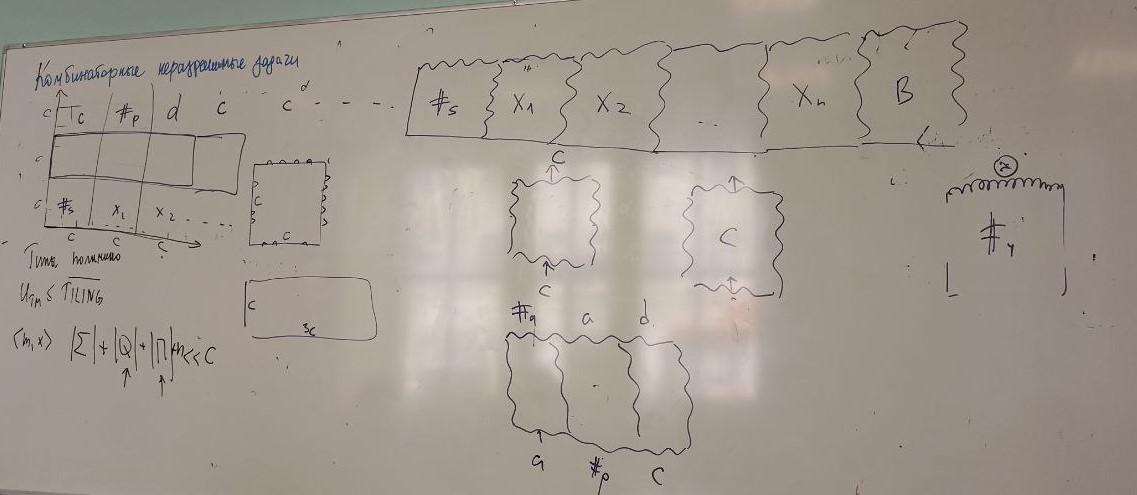
\includegraphics[scale=0.35]{img/polymyno_MT.jpg}
\end{proof}
